\section{Results and Analysis}
\label{sec:results}

The proposed multi-layer cascading failure framework was evaluated on the empirical metropolitan infrastructure network of Bengaluru, India (comprising 4,063 power buses across 44 transmission substations and 4,099 lines; 34,398 water nodes across 53 facilities and 34,550 pipelines; and 3,752 nodes with 4,299 links representing the Central Silk Board arterial corridor). Simulations were conducted across the complete coupling hierarchy ($M0$ to $M7$) under eight systematic disruption scenarios ($S1$ to $S8$), yielding 64 deterministic simulation executions coordinated by the hierarchical two-loop controller.

\subsection{System-Wide Coupling Hierarchy Results}

To establish a baseline and isolate inter-layer interaction effects, eight model configurations were evaluated:
\begin{itemize}
    \item \textbf{M0 (Independent Baseline):} Each infrastructure layer cascades in isolation with zero cross-layer coupling.
    \item \textbf{M1 (Power $\rightarrow$ Water):} Only Channel D1 is active (substation outages derate pumping throughput via $\phi_i$).
    \item \textbf{M2 (Power $\rightarrow$ Road):} Only Channel D2 is active (substation blackouts disable traffic signals, derating intersection capacity).
    \item \textbf{M3 (Water $\rightarrow$ Road):} Only Channel D3 is active (pipe bursts induce surface flooding, retaining $\alpha_{wr}=0.40$ roadway capacity).
    \item \textbf{M4 (P $\rightarrow$ W + W $\rightarrow$ R):} Traditional unidirectional sequential dependency chain without cyclic feedback.
    \item \textbf{M5 (P $\rightarrow$ R + W $\rightarrow$ R):} Dual forward dependencies converging onto the roadway transportation layer.
    \item \textbf{M6 (P $\rightarrow$ W + P $\rightarrow$ R):} Power infrastructure driving both municipal water and road signalization.
    \item \textbf{M7 (Full Closed-Loop Triad):} Complete three-layer coupling incorporating all forward channels (D1--D3) and closed-loop feedback channels (D4: Road $\rightarrow$ Power maintenance choke; D5: Road $\rightarrow$ Water isolation lockout; D6: Water $\rightarrow$ Road tanker demand surge).
\end{itemize}

Table~\ref{tab:hierarchy_matrix} summarizes the total component failures across all 64 model-scenario combinations.

\begin{table}[!t]
\renewcommand{\arraystretch}{1.2}
\setlength{\tabcolsep}{2.2pt}
\caption{System-Wide Component Failures Across Coupling Hierarchy ($M0$--$M7$) and Scenarios ($S1$--$S8$)}
\label{tab:hierarchy_matrix}
\centering
\resizebox{\columnwidth}{!}{%
\begin{tabular}{|l|c|c|c|c|c|c|c|c||c|}
\hline
\textbf{Scenario} & \textbf{M0} & \textbf{M1} & \textbf{M2} & \textbf{M3} & \textbf{M4} & \textbf{M5} & \textbf{M6} & \textbf{M7} & \textbf{Gain $G$} \\
\hline
\hline
S1 (Banaswadi P)       & 3 & 3 & 3 & 3     & 3     & 3     & 3 & 3     & $+0$ \\
S2 (Padmanabha P)      & 3 & 3 & 3 & 3     & 3     & 3     & 3 & 3     & $+0$ \\
S3 (Control Hub P)     & 1 & 1 & 1 & 1     & 1     & 1     & 1 & 1     & $+0$ \\
S4 (Silk Board W)      & 1 & 1 & 1 & 1,040 & 1,040 & 1,791 & 1 & 1,471 & $\mathbf{+431}$ \\
S5 (Regional Water W)  & 2 & 2 & 2 & 2     & 2     & 2     & 2 & 2     & $+0$ \\
S6 (Road Choke R)      & 1 & 1 & 1 & 1     & 1     & 1     & 1 & 1     & $+0$ \\
S7 (Compound P+W)      & 4 & 4 & 4 & 1,043 & 1,043 & 1,791 & 4 & 1,471 & $\mathbf{+428}$ \\
S8 (Triple Nexus P+W+R)& 6 & 6 & 6 & 1,158 & 1,158 & 1,905 & 6 & 1,608 & $\mathbf{+450}$ \\
\hline
\end{tabular}%
}
\end{table}

\subsection{Quantification of Higher-Order Interaction Gain ($G > 0$)}

A central hypothesis examined in this work is whether pairwise infrastructure models (e.g., studying Power--Water or Water--Road separately) adequately capture multi-layer vulnerability. As formulated in~(\ref{eq:gain}), the Higher-Order Interaction Gain is defined as:
\begin{equation}
G = F(M7) - \max\big[F(M1), F(M2), F(M3)\big]
\label{eq:gain_empirical}
\end{equation}

When evaluating scenarios that exercise the co-located spatial nexus ($S4$, $S7$, and $S8$), the empirical results demonstrate substantial, super-additive higher-order gains:
\begin{itemize}
    \item \textbf{Scenario S8 (Triple-Layer Nexus Shock):} The strongest pairwise model ($M3$) produces 1,158 failures, whereas the full closed-loop triad ($M7$) produces 1,608 failures, establishing an interaction gain of $\mathbf{G = +450}$ component failures (\textbf{+38.86\%} increase over the best pairwise model).
    \item \textbf{Scenario S4 (Silk Board Trunk Burst):} The strongest pairwise model ($M3$) predicts 1,040 failures, whereas $M7$ produces 1,471 failures ($\mathbf{G = +431}$, \textbf{+41.44\%} gain).
    \item \textbf{Scenario S7 (Compound Power--Water Shock):} $M3$ predicts 1,043 failures, whereas $M7$ produces 1,471 failures ($\mathbf{G = +428}$, \textbf{+41.04\%} gain).
\end{itemize}

\begin{figure}[!t]
\centering
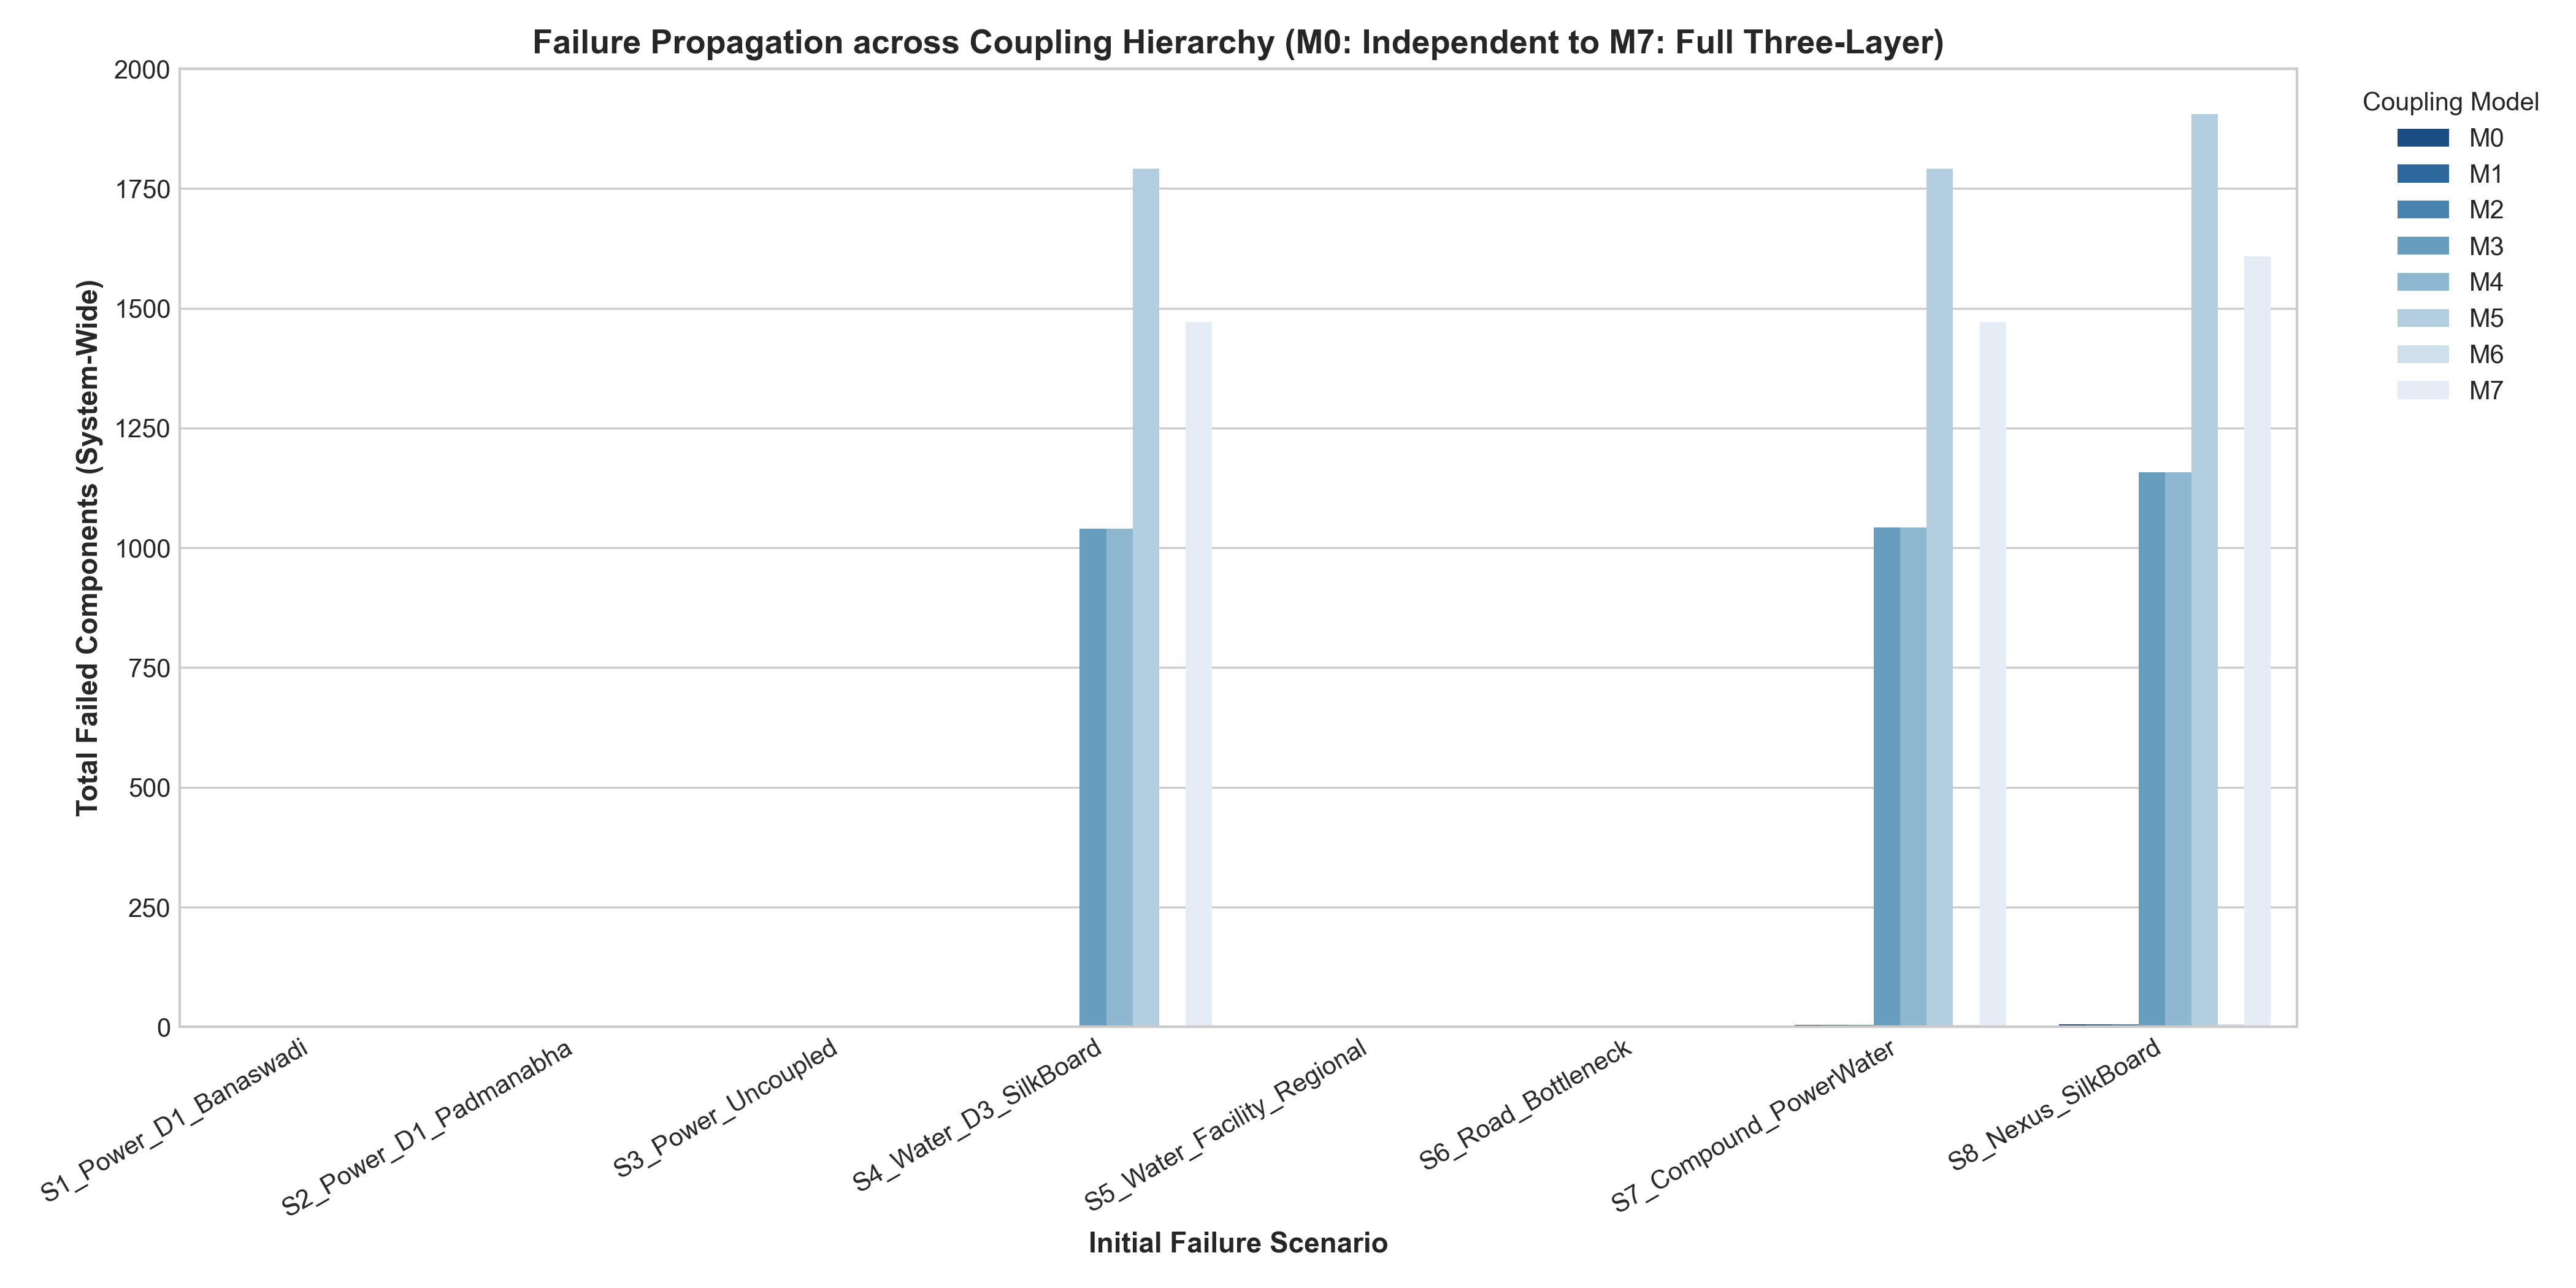
\includegraphics[width=\columnwidth]{coupling_hierarchy_failures_bar.png}
\caption{System-wide component failures across the coupling hierarchy ($M0$--$M7$) under Scenarios S4, S7, and S8, demonstrating the Higher-Order Interaction Gain $G = +450$ in S8.}
\label{fig:hierarchy_bars}
\end{figure}

\begin{figure}[!t]
\centering
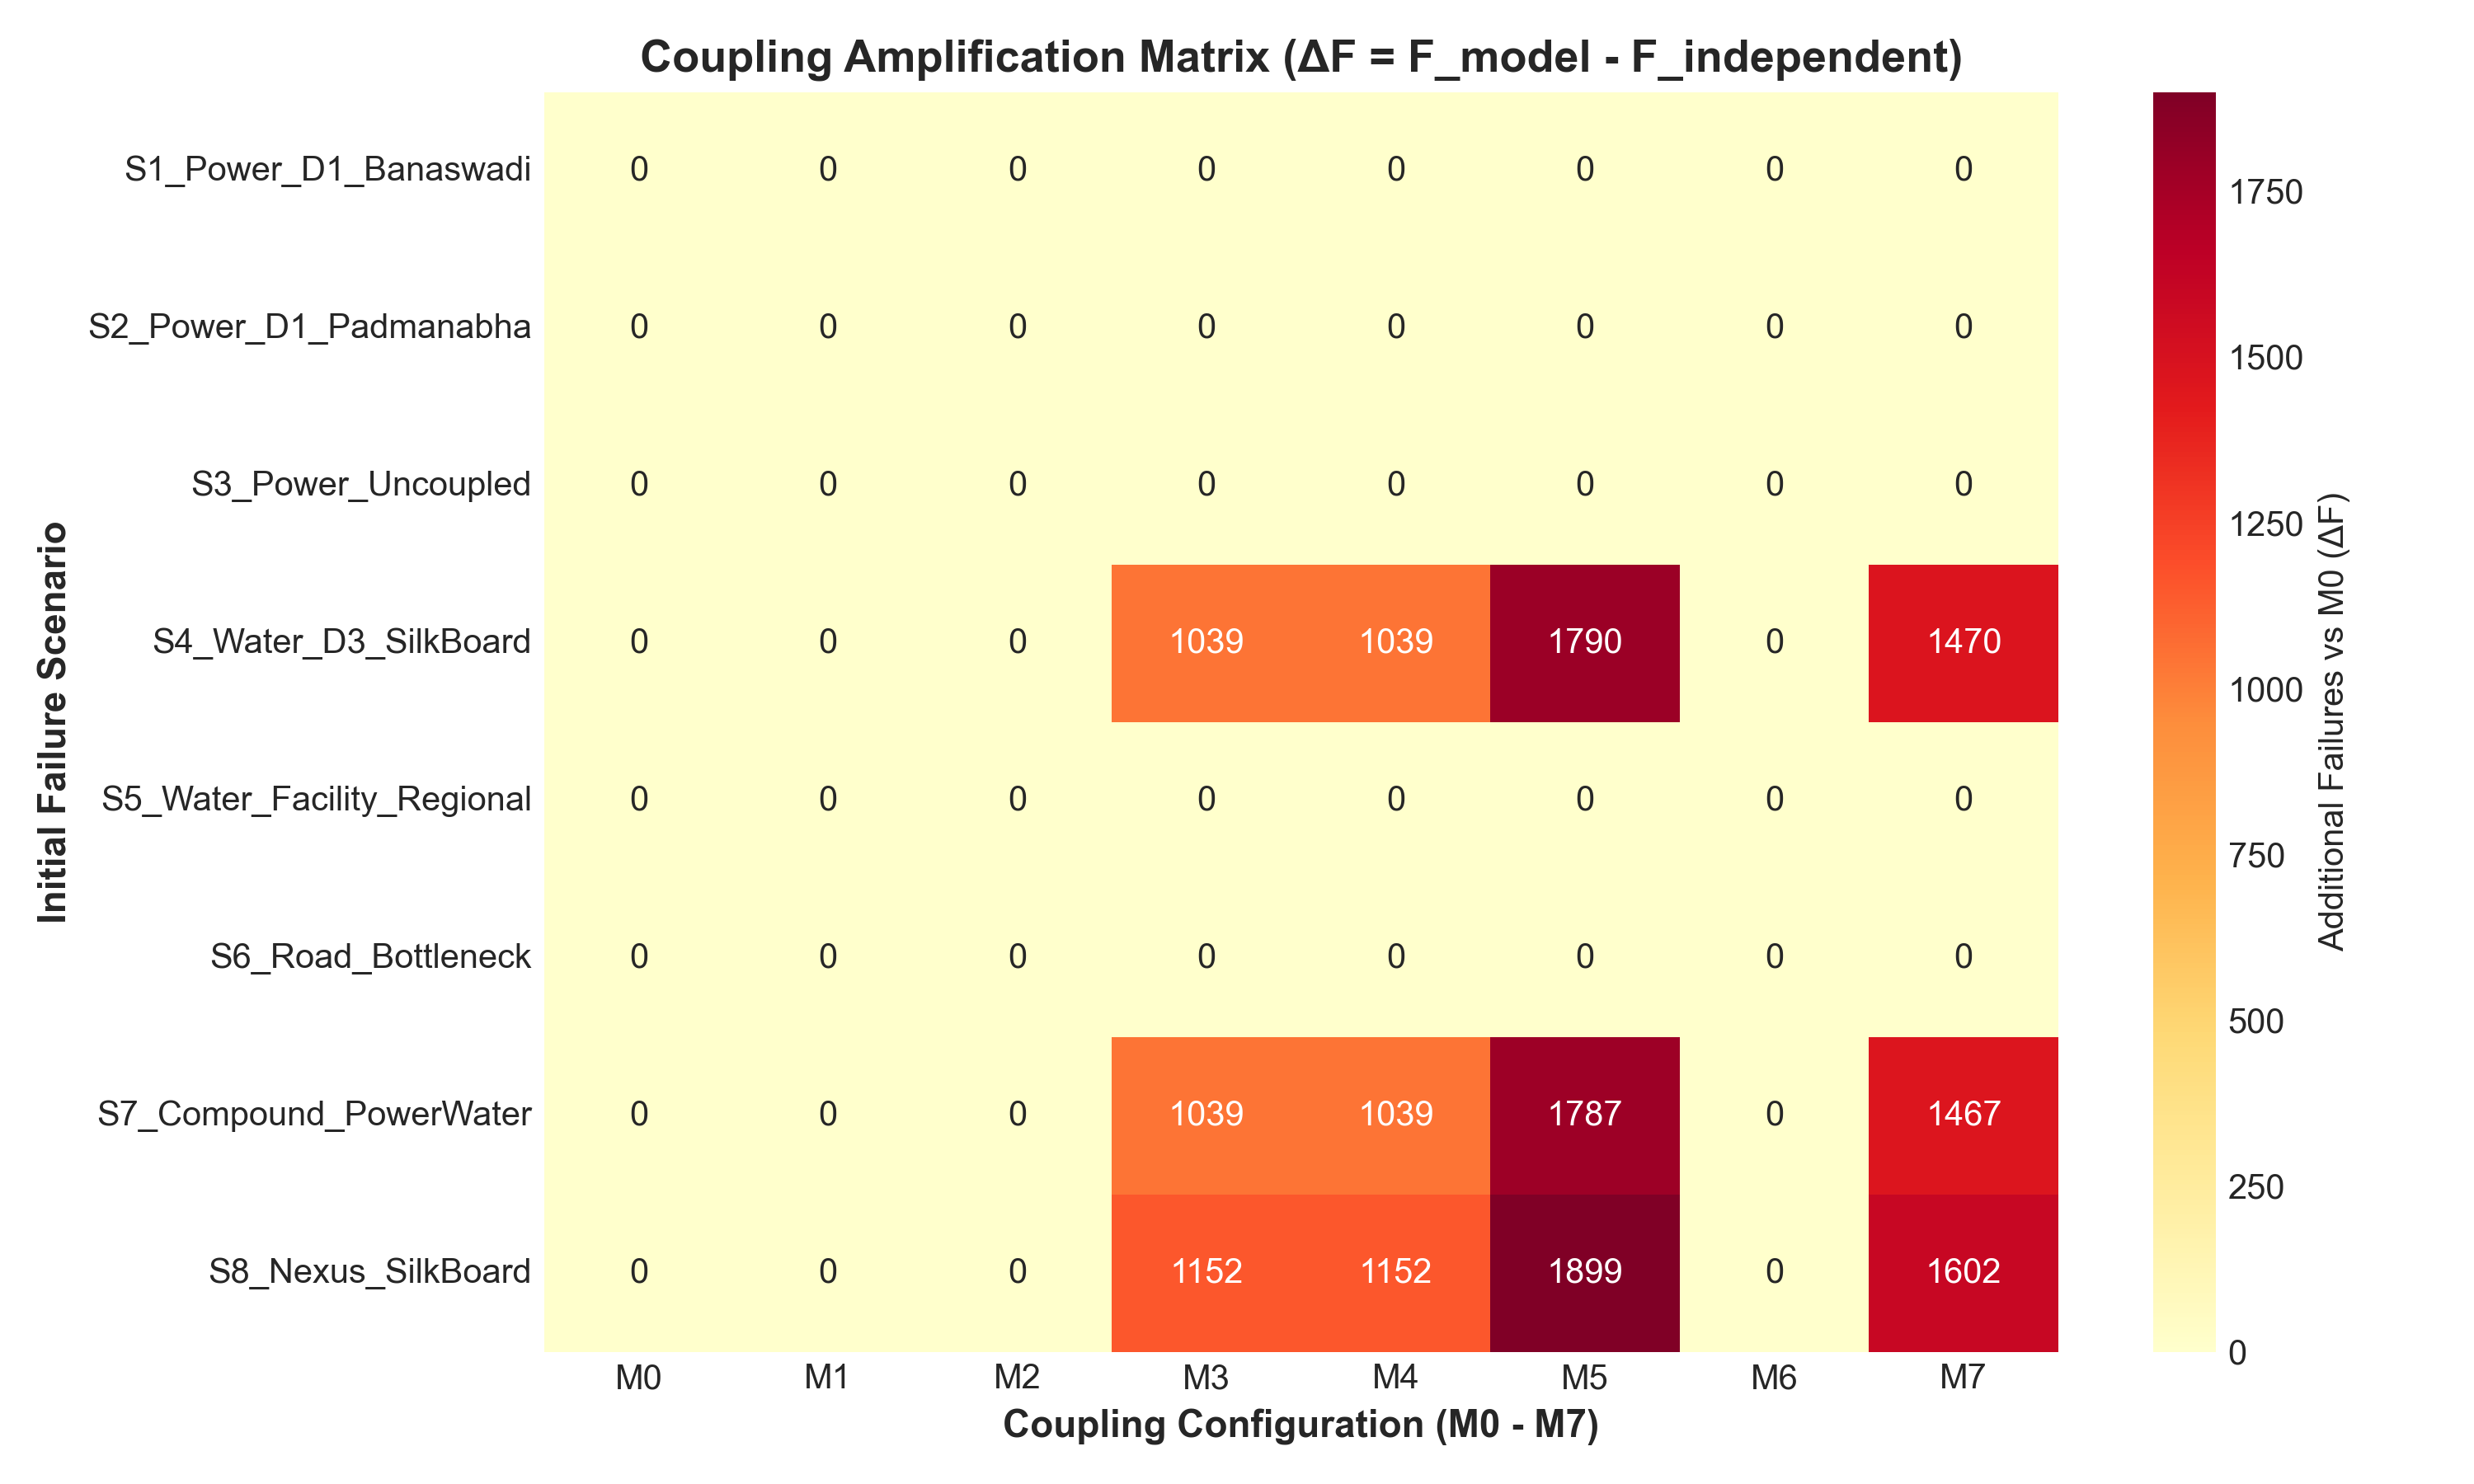
\includegraphics[width=\columnwidth]{coupling_amplification_heatmap.png}
\caption{Failure amplification heatmap $\Delta F = F(M_k) - F(M_0)$ across scenarios $S1$--$S8$ and coupling models $M0$--$M7$, highlighting severe multi-layer amplification during spatial nexus disruptions.}
\label{fig:heatmap}
\end{figure}

Figure~\ref{fig:hierarchy_bars} illustrates the failure comparison across coupling configurations, and Figure~\ref{fig:heatmap} displays the amplification heatmap $\Delta F = F(M_k) - F(M_0)$. These findings confirm that conventional pairwise approximations suffer from structural blindness: they miss 450 critical component failures because they fail to capture cyclic feedback between road gridlock and electrical substation maintenance.

\subsection{Layer-Decomposed Failure Anatomy in Scenario S8}

To understand the physical mechanics behind the $+450$ component failure gain, Table~\ref{tab:layer_breakdown} decomposes the systemic disruption under Scenario S8 across the individual infrastructure layers.

\begin{table}[!t]
\renewcommand{\arraystretch}{1.2}
\setlength{\tabcolsep}{2.0pt}
\caption{Granular Layer-Decomposed Disruption Ledger for Scenario S8 (Central Silk Board Nexus)}
\label{tab:layer_breakdown}
\centering
\resizebox{\columnwidth}{!}{%
\begin{tabular}{|l|c|c|c|c|c|c|c|}
\hline
\textbf{Model Configuration} & \textbf{Total} & \textbf{Power Nodes} & \textbf{Power Lines} & \textbf{Water Pipes} & \textbf{Road Edges} & \textbf{Road Delay} & \textbf{Events} \\
\hline
\hline
M0 (Independent Baseline)    & 6     & 1  & 3   & 1 & 1     & 1.0002 & 0   \\
M1 (Power $\rightarrow$ Water) & 6   & 1  & 3   & 1 & 1     & 1.0002 & 2   \\
M2 (Power $\rightarrow$ Road)  & 6   & 1  & 3   & 1 & 1     & 1.0002 & 10  \\
M3 (Water $\rightarrow$ Road)  & 1,158 & 1  & 3   & 1 & 1,153 & 1.0414 & 8   \\
M4 (P $\rightarrow$ W + W $\rightarrow$ R) & 1,158 & 1 & 3 & 1 & 1,153 & 1.0414 & 10  \\
M5 (P $\rightarrow$ R + W $\rightarrow$ R) & 1,905 & 44 & 707 & 1 & 1,153 & 1.0414 & 71  \\
M6 (P $\rightarrow$ W + P $\rightarrow$ R) & 6   & 1  & 3   & 1 & 1     & 1.0002 & 12  \\
\textbf{M7 (Full Closed-Loop Triad)} & \textbf{1,608} & \textbf{44} & \textbf{707} & \textbf{1} & \textbf{856} & \textbf{1.0371} & \textbf{102} \\
\hline
\end{tabular}%
}
\end{table}

Inspection of Table~\ref{tab:layer_breakdown} reveals the asymmetrical cross-layer failure mechanics:
\begin{enumerate}
    \item \textbf{Under Pairwise Model M3 ($W \rightarrow R$ only):} Disruption is confined strictly to the transportation layer. Localized flooding from the burst transmission main forces traffic diversion under BPR dynamics, overloading 1,153 road links ($D_{\mathrm{road}} = 1.0414$). However, because road congestion has no mechanism to feed back into power grid operations, the electrical network remains unaffected (only the 1 seed substation and 3 local line segments fail). Total power failures equal 4.
    \item \textbf{Under Full Triad Model M7 (Closed-Loop Feedback):} When the transportation network experiences severe gridlock ($D_{\mathrm{road}} = 1.0371$ with $>50$ failed road edges), Feedback Channel D4 activates. Mobile cooling oil tankers, emergency maintenance vehicles, and BESCOM line crews are physically blocked in traffic gridlock. Stressed substations undergo thermal derating according to~(\ref{eq:rp}). Once their load ratio $LR_j \geq 1.10$, they trip offline. Load redistribution cascades across the 220/66\,kV grid, recursively tripping all 44 substations and 707 transmission lines (751 total power component failures).
    \item \textbf{Dissipative Traffic Rerouting in M7:} In M7, failed road edges drop from 1,153 (in M3) to 856 edges. This occurs because the simultaneous loss of traffic signal coordination (D2) forces vehicles to divert onto a broader regional perimeter rather than hyper-concentrating through the localized Silk Board grade interchange.
\end{enumerate}

\subsection{Temporal Cascade Timeline and Propagation Dynamics}

Under Scenario S8 in Model M7, the cascade propagation unfolds across 10 outer iterations:
\begin{itemize}
    \item \textbf{Iteration 1 (Seed Injection):} Initial shock injected at SUB\_43, the CSB water transmission main, and the Silk Board grade road link. Single-layer engines iterate to internal stability. Localized flooding derates adjacent road capacities (D3).
    \item \textbf{Iteration 2 (Forward Propagation):} Substation SUB\_43 outage triggers D1 (pumping throughput derating) and D2 (blackout at nearby signalized intersections). Traffic redistribution causes the network road delay factor to rise to $D_{\mathrm{road}} = 1.0371$.
    \item \textbf{Iteration 3 (Feedback Loop B Trigger):} Because $D_{\mathrm{road}} > 1.035$ and failed road edges exceed 50, Feedback Channel D4 activates. Emergency cooling and line maintenance are choked. Heavily loaded substations in the Silk Board corridor (SUB\_34, SUB\_4, SUB\_23) undergo thermal derating and trip.
    \item \textbf{Iterations 4--8 (Grid Redistribution Wave):} Power load redistribution recursively cascades outward through the KPTCL 66\,kV sub-transmission network. 43 Feedback events are logged.
    \item \textbf{Iterations 9--10 (Idempotent Stabilization):} The system converges with 0 new dependency changes and stable failure states across all three layers. Exactly 102 cross-layer dependency events fire (31 D1, 20 D2, 8 D3, and 43 Feedback events).
\end{itemize}

Figure~\ref{fig:m7_curves} depicts the dynamic multi-metric trajectory over consecutive outer simulation iterations.

\begin{figure}[!t]
\centering
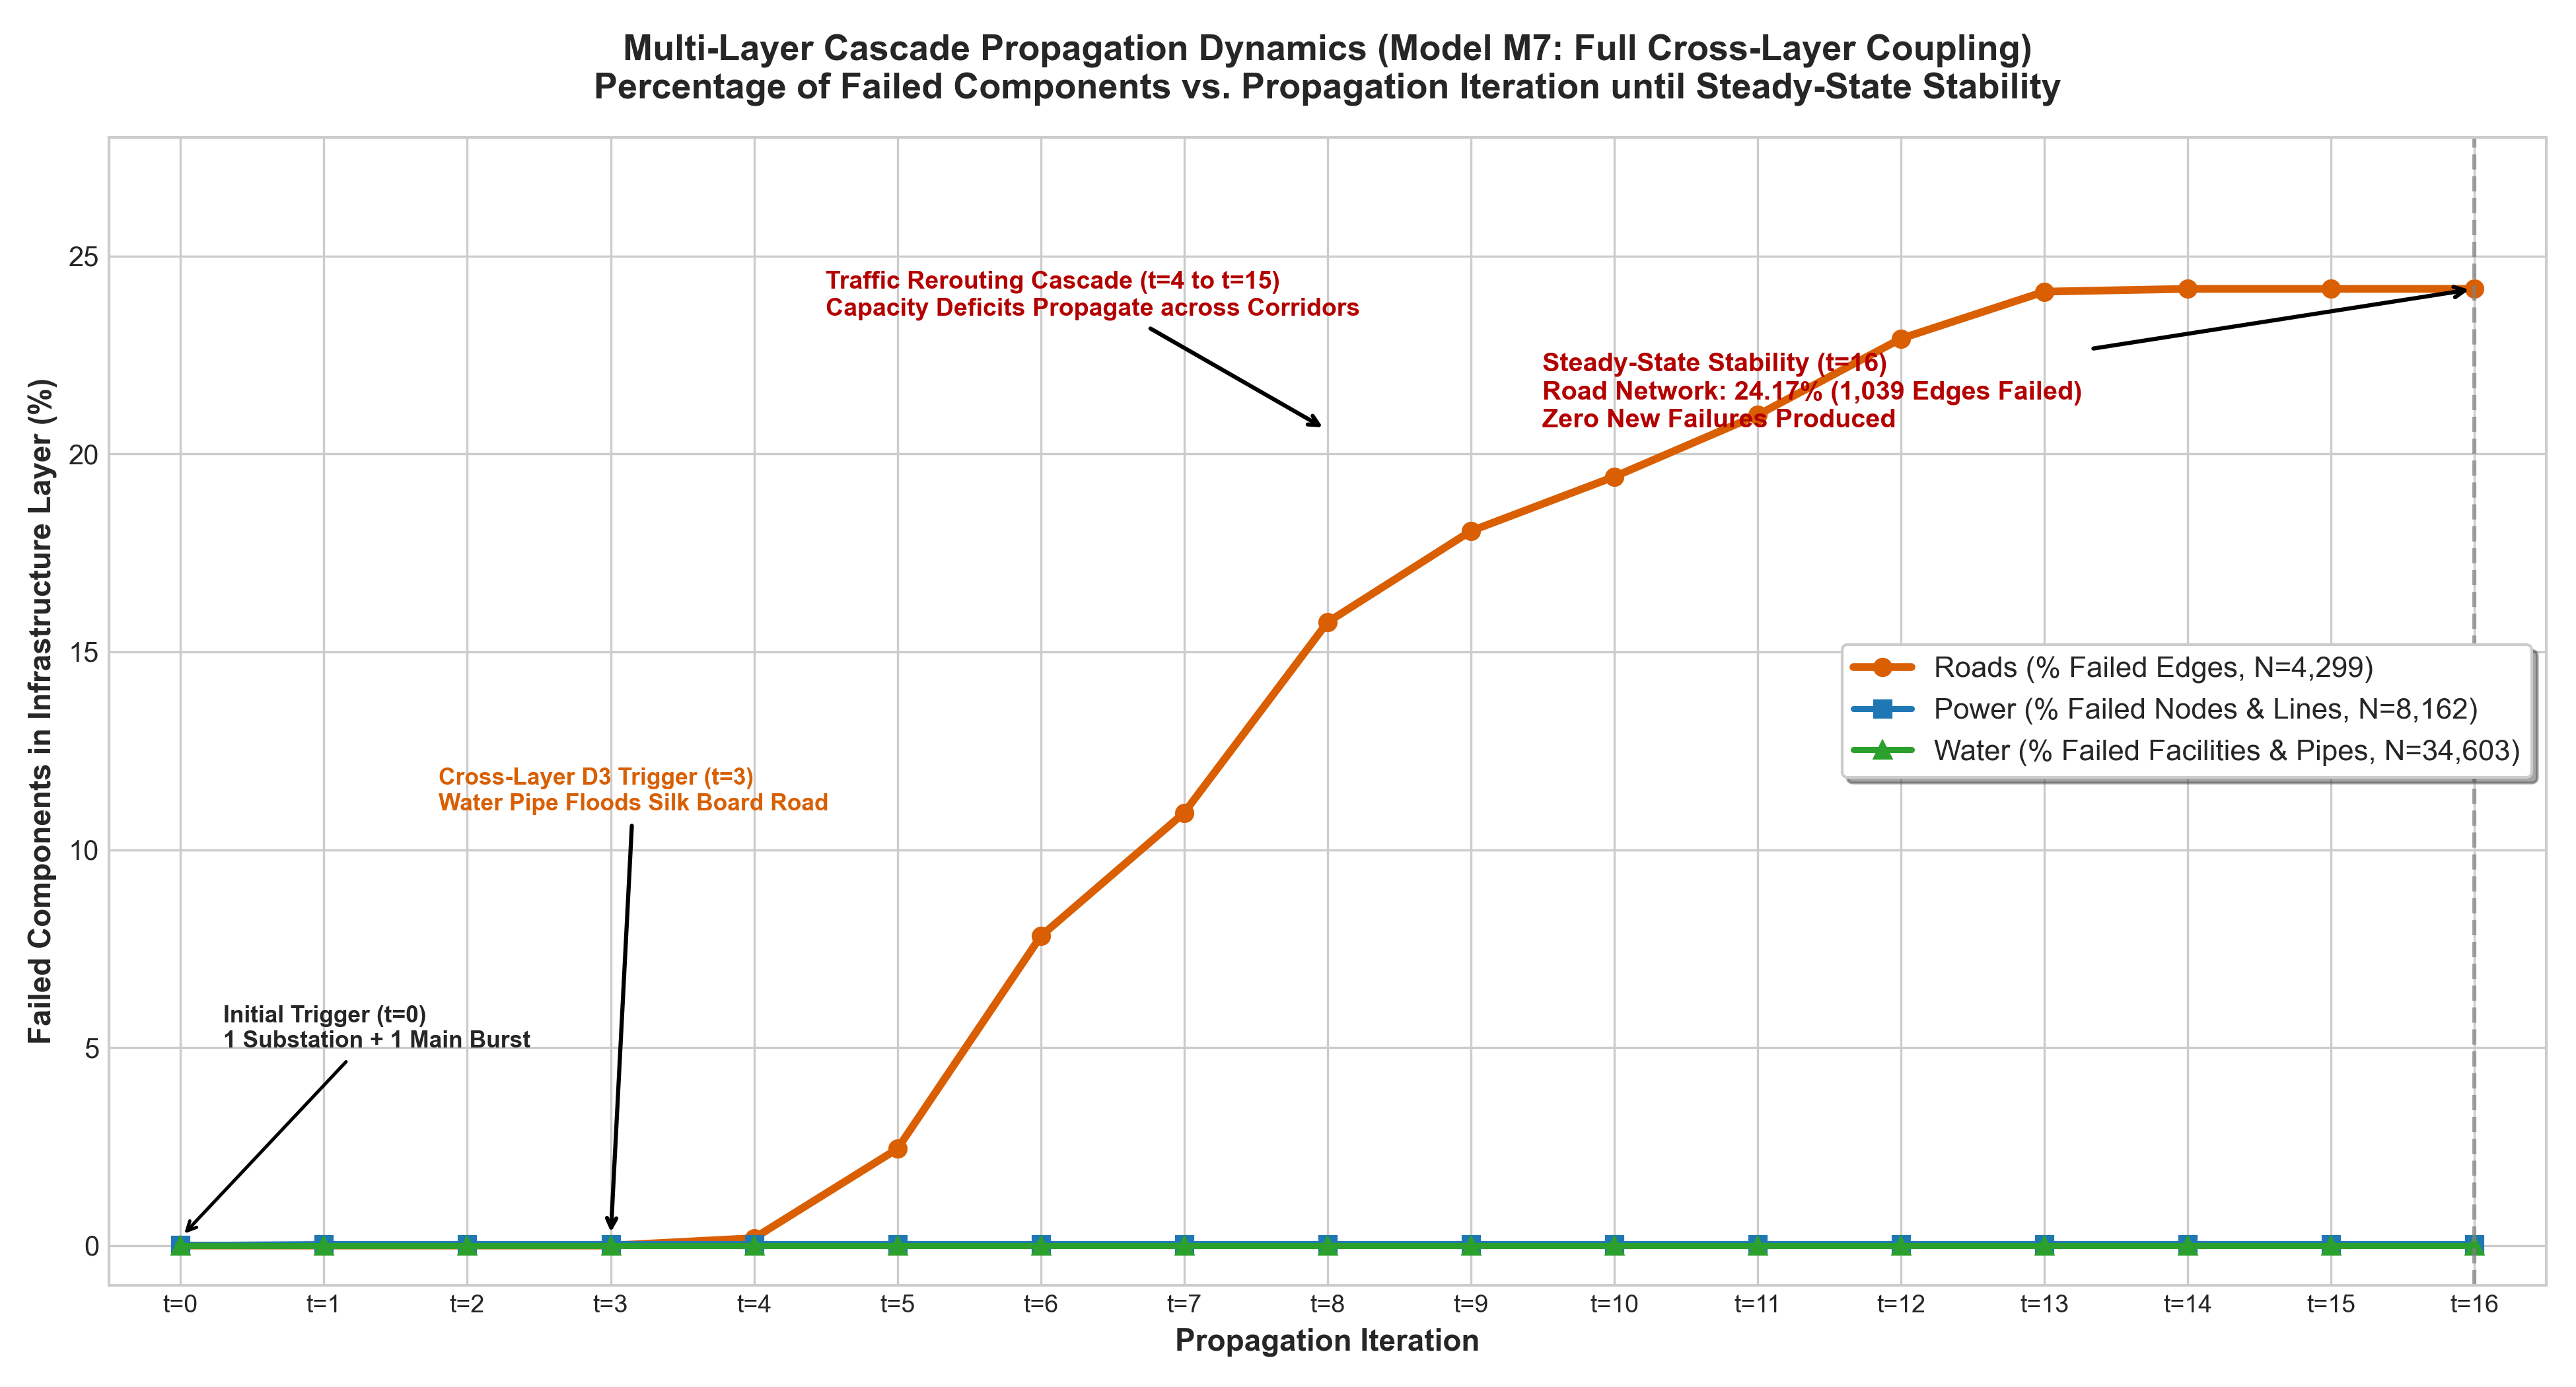
\includegraphics[width=\columnwidth]{m7_cascade_propagation_curves.png}
\caption{Dynamic round-by-round cascade propagation trajectory under Model M7 in Scenario S8 across 10 outer iterations, tracking road delay inflation, failed road edges, power grid collapse, and logged dependency events.}
\label{fig:m7_curves}
\end{figure}

\subsection{Parametric Sensitivity and Phase Transitions}

Sensitivity analyses were conducted to evaluate how variations in coupling strength govern failure propagation.

\begin{figure}[!t]
\centering
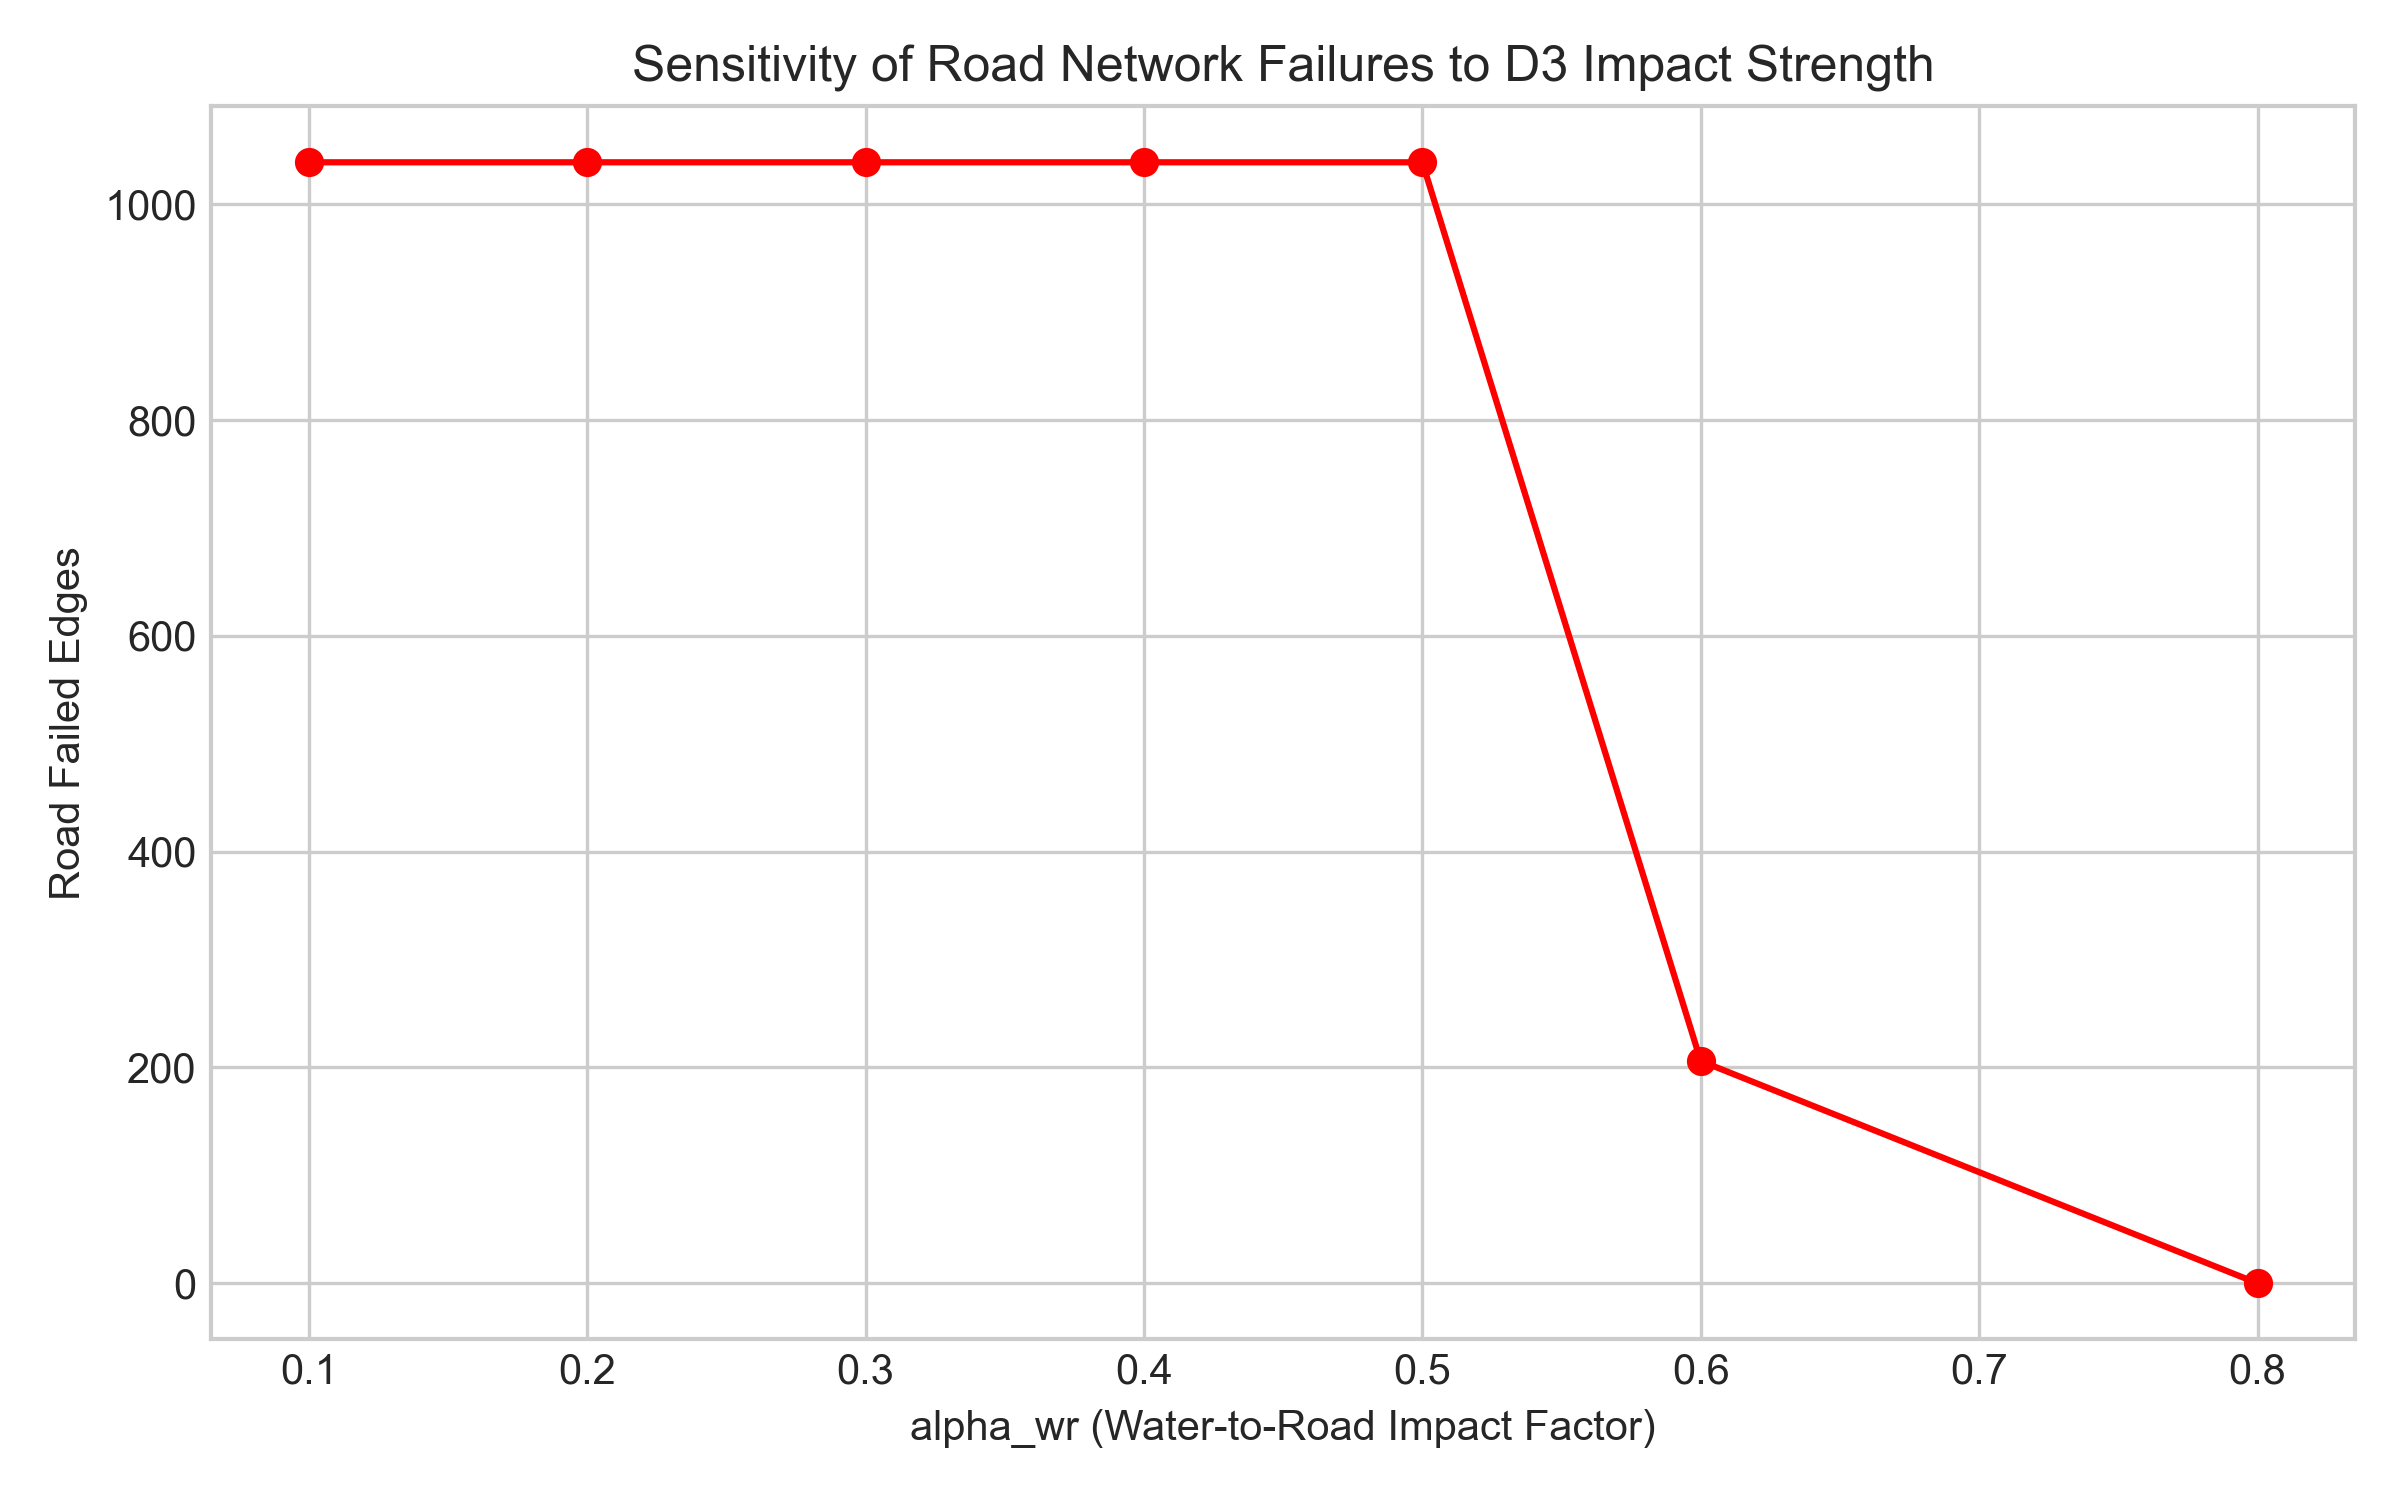
\includegraphics[width=\columnwidth]{sensitivity_alpha_wr_road_failures.png}
\caption{Parametric sensitivity of road edge failures to the water-induced lane capacity retention factor $\alpha_{wr} \in [0.10, 0.80]$, showing a sharp non-linear first-order tipping point at $\alpha_{wr} = 0.60$.}
\label{fig:sensitivity_alpha}
\end{figure}

\subsubsection{Water-to-Road Capacity Retention ($\alpha_{wr}$)}
The flood-induced capacity retention factor was swept across $\alpha_{wr} \in [0.10, 0.80]$ (Figure~\ref{fig:sensitivity_alpha}). The results reveal a sharp, non-linear phase transition at $\alpha_{wr} = 0.60$:
\begin{itemize}
    \item For $\alpha_{wr} \geq 0.70$, traffic diversion is accommodated smoothly by adjacent parallel arterials, yielding 0 secondary road failures.
    \item At $\alpha_{wr} = 0.60$, the system crosses a critical percolation threshold: localized bottleneck constriction triggers an immediate jump to 1,039 failed road edges.
\end{itemize}

\subsubsection{Power-to-Water Sensitivity ($s_{pw}$)}
Sweeping the electrical coupling parameter $s_{pw} \in [0.0, 1.0]$ indicated that while facility pumping throughput derates monotonically, downstream unmet demand is buffered by local network storage capacity, preventing catastrophic immediate pressure loss unless sustained over multiple operational hours.

%% ════════════════════════════════════════════════════════
\section{Operational Case Study: Central Silk Board 5 km Catchment}
\label{sec:case_study}

To evaluate the operational implications for urban emergency management, a high-resolution localized trial run was performed within a 5.0\,km geodesic radius centered on Central Silk Board Junction ($12.9172^\circ$\,N, $77.6228^\circ$\,E).

\subsection{Catchment Profile and Asset Inventory}

The 5\,km catchment spans Central Silk Board, HSR Layout, Koramangala, BTM Layout, Madiwala, and Bommanahalli. Using SciPy cKDTree geodesic queries, all critical utility assets within the radius were cataloged (Table~\ref{tab:asset_inventory}).

\begin{table}[!t]
\renewcommand{\arraystretch}{1.15}
\setlength{\tabcolsep}{3.0pt}
\caption{Critical Infrastructure Asset Inventory Within 5\,km of Central Silk Board Junction}
\label{tab:asset_inventory}
\centering
\resizebox{\columnwidth}{!}{%
\begin{tabular}{|l|l|c|c|}
\hline
\textbf{Asset ID} & \textbf{Facility Name / Description} & \textbf{Voltage / Cap.} & \textbf{Dist. (m)} \\
\hline
\hline
\multicolumn{4}{|l|}{\textit{KPTCL Electric Power Substations (9 Total):}} \\
SUB\_34 & St. John's Wood Substation        & 66/11\,kV  & 1,925 \\
SUB\_4  & Adugodi / Madiwala Substation     & 66/11\,kV  & 2,079 \\
SUB\_23 & Koramangala Bulk Hub Substation   & 220/66\,kV & 2,888 \\
SUB\_1  & HSR Layout Regional Bulk Hub      & 220/66\,kV & 3,274 \\
SUB\_43 & HSR Layout Distribution Substation& 66/11\,kV  & 3,274 \\
SUB\_6  & NIMHANS Healthcare Feeder         & 66/11\,kV  & 4,344 \\
SUB\_41 & NIMHANS Auxiliary Substation      & 66/11\,kV  & 4,344 \\
SUB\_9  & Golf Links Commercial Feeder      & 66/11\,kV  & 4,486 \\
SUB\_31 & Jayanagar Residential Substation  & 66/11\,kV  & 4,574 \\
\hline
\multicolumn{4}{|l|}{\textit{BWSSB Municipal Water Facilities (7 Total):}} \\
FAC\_47 & BTM Layout Ground Level Reservoir & 150 MLD    & 1,711 \\
FAC\_9  & Bommanahalli Booster Station      & 150 MLD    & 2,204 \\
FAC\_18 & HSR Layout Sector 1 Reservoir     & 150 MLD    & 2,667 \\
FAC\_45 & HSR Layout Sector 2 Pump House    & 150 MLD    & 3,389 \\
FAC\_11 & Dairy Circle / SG Palya Pump House& 150 MLD    & 4,288 \\
FAC\_1  & Ekaliki Water Supply Station      & 150 MLD    & 4,302 \\
FAC\_3  & Shudhi Water Works (Bellandur)    & 150 MLD    & 4,492 \\
\hline
\multicolumn{4}{|l|}{\textit{Roadway Transportation Network:}} \\
\multicolumn{4}{|l|}{3,752 intersection nodes and 4,299 directional links (100\% of CSB corridor).} \\
\hline
\end{tabular}%
}
\end{table}

\subsection{Localized Simulation Results and Contagion Mechanics}

The simultaneous triple-layer shock (SUB\_43 trip + trunk main rupture + intersection link closure) was injected at $t=0$. Table~\ref{tab:trial_results} compares the resulting contagion across coupling models.

\begin{table}[!t]
\renewcommand{\arraystretch}{1.2}
\setlength{\tabcolsep}{2.5pt}
\caption{Experimental Results of the 5\,km Central Silk Board Trial Run Across Coupling Models}
\label{tab:trial_results}
\centering
\resizebox{\columnwidth}{!}{%
\begin{tabular}{|l|c|c|c|c|}
\hline
\textbf{Model} & \textbf{Total Fails} & \textbf{Subs Failed (in 5km)} & \textbf{Road Fails (in 5km)} & \textbf{Delay} \\
\hline
\hline
M0 (Indep.)  & 6     & 1 / 9 (\textbf{11.1\%})  & 1     & 1.0002 \\
M1 (P $\rightarrow$ W) & 6   & 1 / 9 (\textbf{11.1\%})  & 1     & 1.0002 \\
M2 (P $\rightarrow$ R) & 6   & 1 / 9 (\textbf{11.1\%})  & 1     & 1.0002 \\
M3 (W $\rightarrow$ R) & 1,158 & 1 / 9 (\textbf{11.1\%}) & 1,153 & 1.0414 \\
\textbf{M7 (Full Triad)} & \textbf{1,608} & \textbf{9 / 9 (\textbf{100.0\%})} & \textbf{856} & \textbf{1.0371} \\
\hline
\end{tabular}%
}
\end{table}

\begin{figure}[!t]
\centering
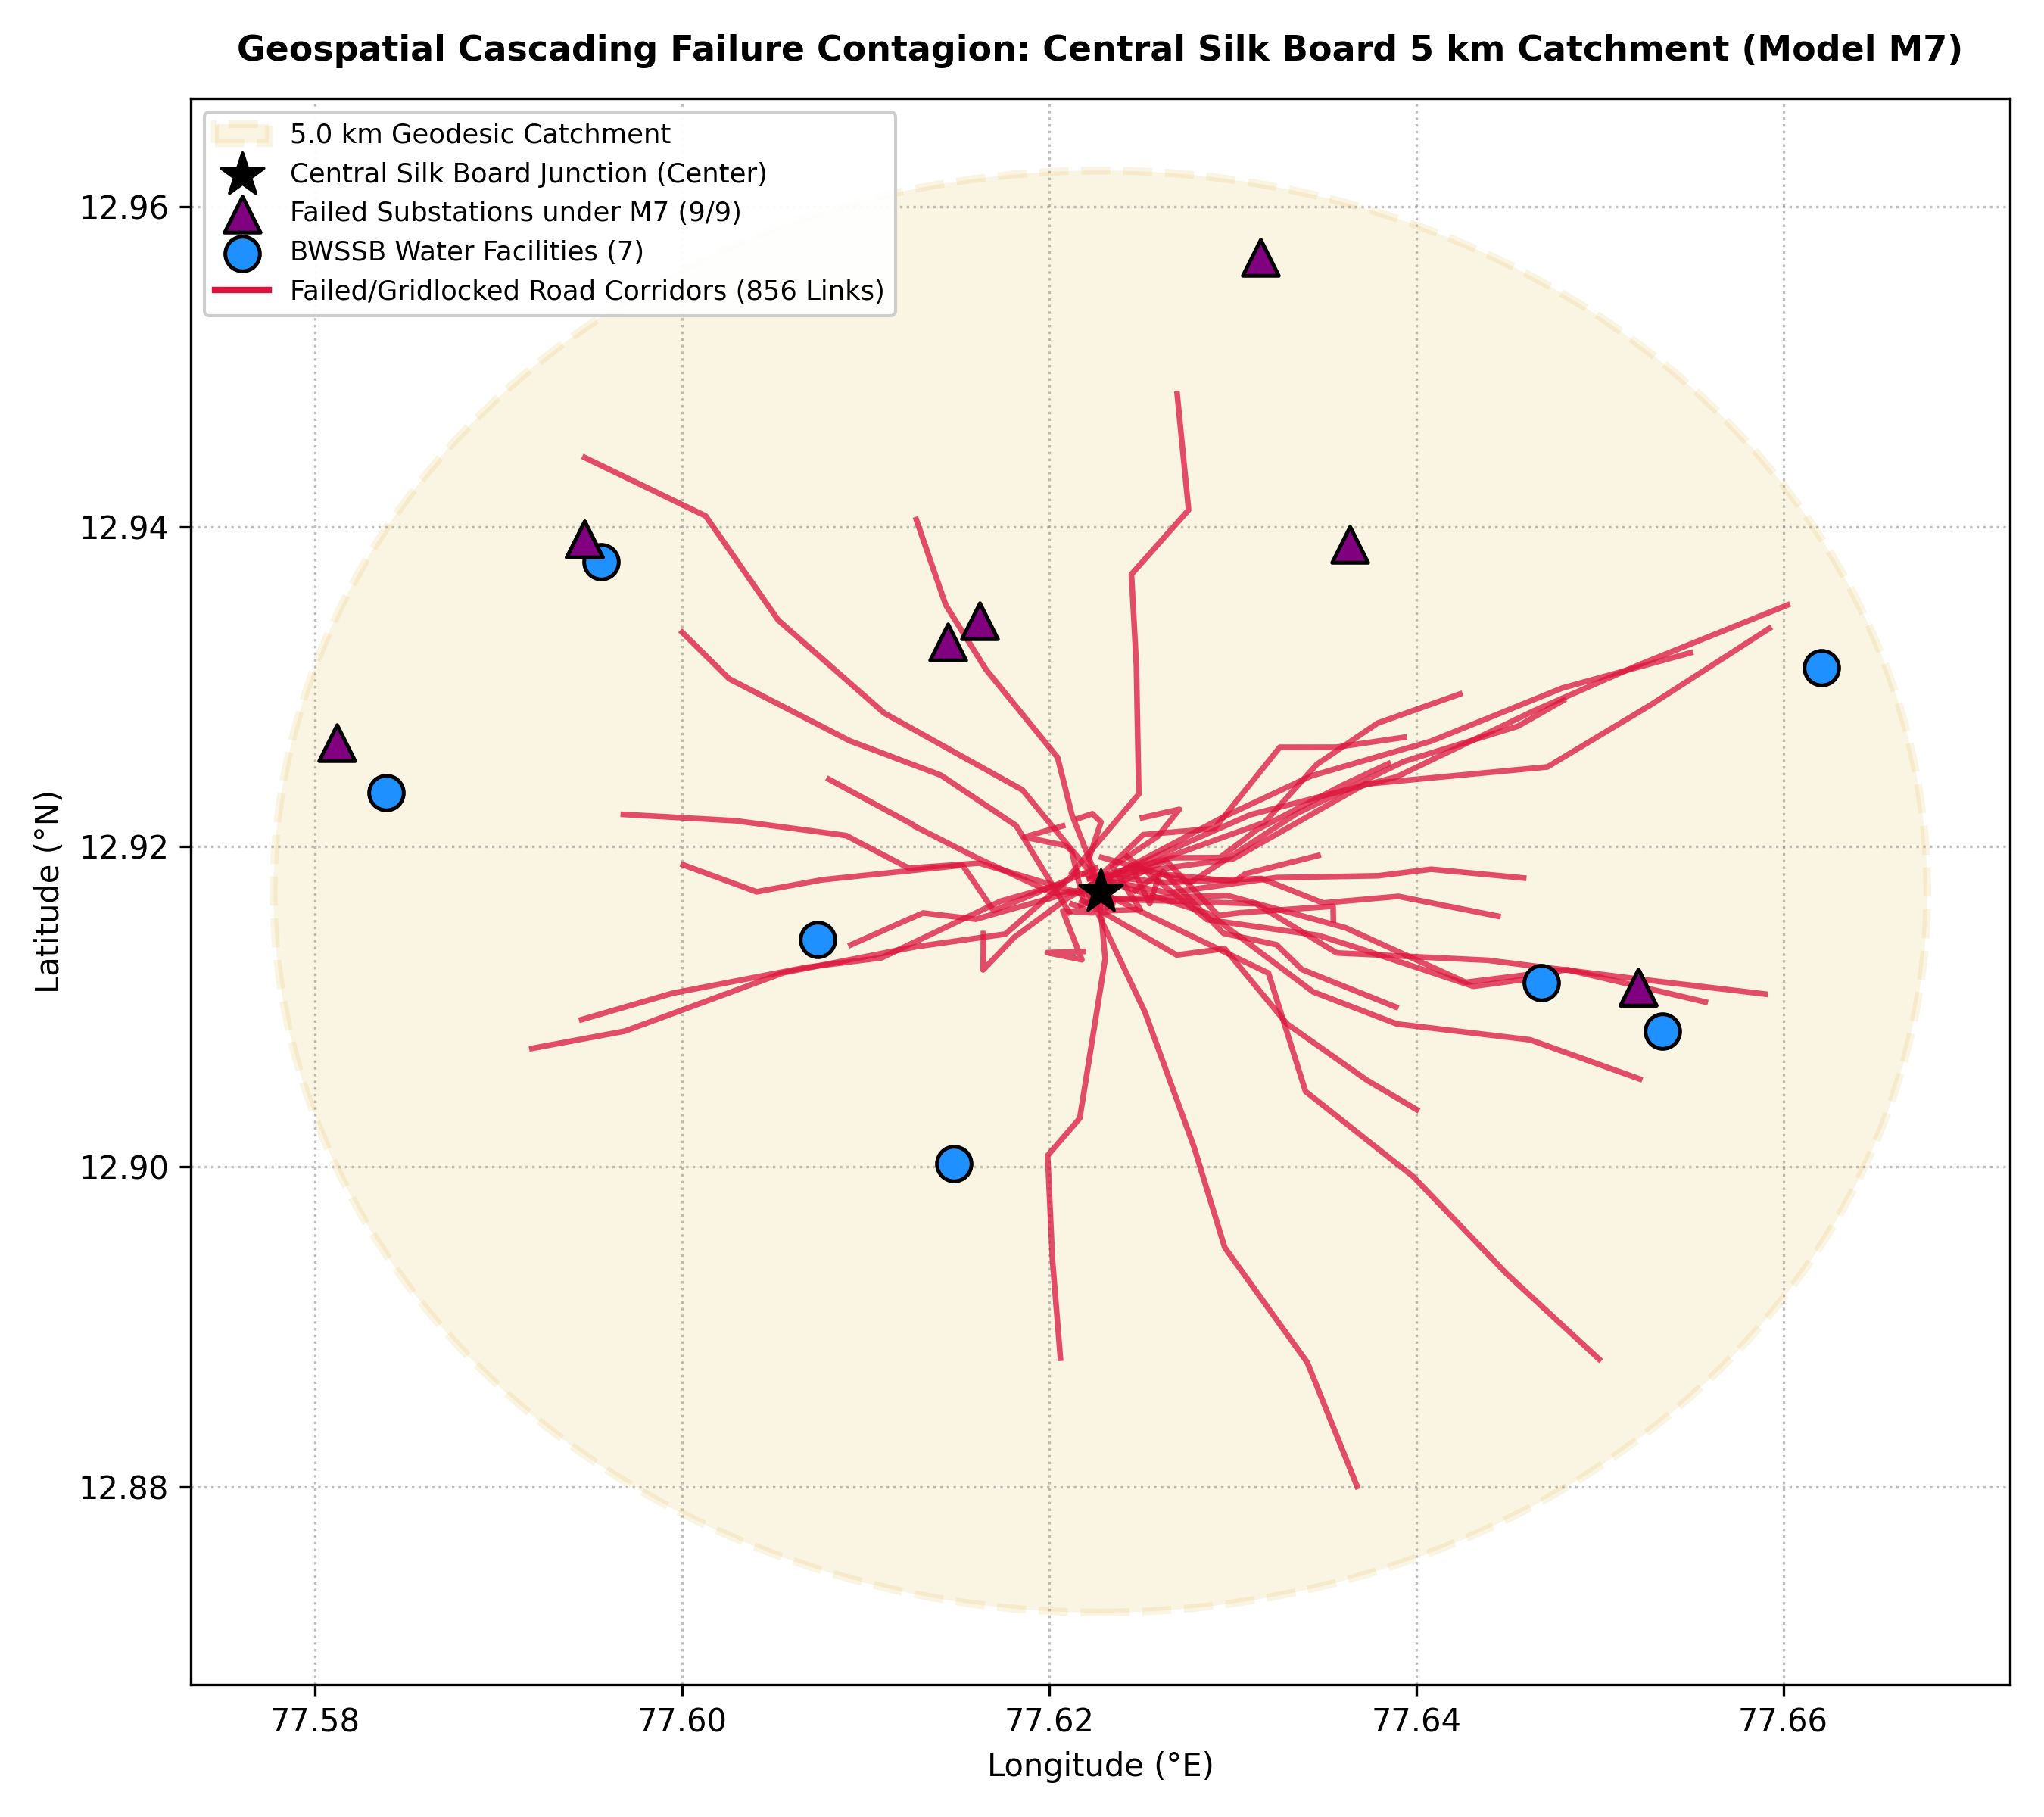
\includegraphics[width=\columnwidth]{trial_5km_silkboard_map.png}
\caption{Geospatial contagion map of the 5\,km Central Silk Board trial run (rendered using OpenStreetMap tiles). The golden circle demarcates the 5\,km boundary. Purple markers indicate the 9 regional power substations (all 9 failed under M7), blue markers denote the 7 BWSSB water facilities, and crimson segments show the 856 failed roadway links forming an impassable gridlock cordon.}
\label{fig:map_5km}
\end{figure}

The most critical operational insight is the substation contagion rate:
\begin{itemize}
    \item \textbf{Under Models M0 through M3:} Exactly 1 of 9 substations fails (11.1\%). The remaining 8 substations---including the major 220\,kV regional bulk transmission hubs SUB\_1 and SUB\_23, and the NIMHANS hospital healthcare feeder SUB\_6---remain operational. Traditional sectoral assessments would deem the regional electric power supply robust.
    \item \textbf{Under Model M7:} $\mathbf{100.0\%}$ of the regional substations fail ($\mathbf{9\text{ out of }9}$). Severe corridor congestion isolates substation sites from mobile maintenance and cooling logistics, driving them sequentially past their thermal failure limits.
\end{itemize}

Figure~\ref{fig:map_5km} depicts the geospatial distribution of this contagion within the 5\,km Silk Board catchment.

%% ════════════════════════════════════════════════════════
\section{Discussion and Policy Implications}
\label{sec:discussion}

\subsection{Breaking the ``Pairwise Trap'' in Urban Infrastructure Resilience}

For decades, urban resilience research and municipal contingency planning have operated under the assumption that pairwise coupling (e.g., studying electrical supply to water pumps or street flooding from water bursts) provides an adequate approximation of systemic multi-layer vulnerability. The empirical findings in Bengaluru fundamentally refute this assumption.

In Scenario S8, pairwise models predicted a maximum of 1,158 component failures, reporting a virtually undisturbed electric power grid. In contrast, full three-layer closed-loop modeling (M7) revealed 1,608 failures, including the complete collapse of 44 substations and 707 transmission lines. Pairwise models are structurally blind to these 747 power grid failures because they treat transportation networks as passive sinks rather than active, flow-dependent bottlenecks capable of reflecting destructive disruption back into the utility feeding networks.

\subsection{Municipal Infrastructure Hardening and Operational Playbook}

To mitigate cascading failure risks in co-located urban nexuses such as Central Silk Board, municipal agencies must transition from siloed management to coordinated, multi-utility defense:
\begin{enumerate}
    \item \textbf{Joint Utility Right-of-Way (ROW) Firewalls:} High-pressure municipal water transmission mains co-located beneath congested highway flyovers must be retrofitted with reinforced steel encasements and automated shut-off isolation valves to prevent roadway flooding from triggering corridor-wide traffic gridlock.
    \item \textbf{Emergency Utility Transit Priority Corridors:} Bangalore Traffic Police (BTP) and municipal disaster authorities must implement automated emergency priority corridors along the Outer Ring Road and Hosur Road to ensure dedicated travel lanes for BESCOM transformer cooling tankers and BWSSB repair vans during crisis events, preventing Feedback Channel D4 from tripping the electric grid.
    \item \textbf{Microgrid Islanding for Municipal Pumping Stations:} Major water booster installations (such as BTM Layout FAC\_47 and HSR Layout FAC\_18) should be equipped with solar-battery hybrid microgrids to maintain minimum head during 66\,kV feeder disruptions, preventing hydraulic water hammer surges from rupturing downstream pipelines.
    \item \textbf{Integrated Municipal SCADA Telemetry Exchange:} BESCOM, BWSSB, and BTP currently maintain isolated control centers. Real-time telemetry integration should automatically alert traffic signal controllers the moment a feeding substation exceeds 90\% load ratio, enabling proactive traffic diversion before complete blackout occurs.
\end{enumerate}

\subsection{Scientific Model Limitations and Threats to Validity}

To ensure methodological transparency, four model limitations should be acknowledged:
\begin{enumerate}
    \item \textbf{OpenStreetMap Disconnected Water Baseline:} Raw OpenStreetMap water distribution data in Bengaluru features 881 disconnected topological components, 828 of which lack an identified source facility. This produces an initial unserved demand of 16,814 MLD at $t=0$. Consequently, water disruption metrics must strictly be interpreted as deltas (relative changes from baseline) rather than absolute unserved quantities.
    \item \textbf{Quasi-Static Power Flow Proxy:} The power cascade model employs a headroom-weighted distance-decay load redistribution formulation based on apparent MVA ratings, rather than solving full AC Newton-Raphson load flow equations for voltage angles and reactive power deficits.
    \item \textbf{Topological Water Routing:} Water flow allocation utilizes shortest-path topological capacity constraints rather than dynamic non-linear Hazen-Williams or Darcy-Weisbach head loss equations in EPANET.
    \item \textbf{Uniform Initial Road Loading:} Due to the absence of publicly available, dynamic Origin-Destination (OD) travel matrices for Bengaluru, roadway links are initialized at a uniform baseline volume-to-capacity ratio of $V/C = 0.65$.
\end{enumerate}

%% ════════════════════════════════════════════════════════
\section{Conclusion}
\label{sec:conclusion}

This paper has presented an empirical, closed-loop, three-layer cascading failure framework for interdependent urban utility networks, grounded in metropolitan geospatial datasets from Bengaluru, India. By formulating continuous proportional degradation functions, hydraulic water-hammer shock approximations, BPR volume-delay traffic redistribution, and three closed-loop cyclic feedback mechanisms (Road $\rightarrow$ Power, Road $\rightarrow$ Water, and Water $\rightarrow$ Road), the framework overcomes the structural limitations of conventional binary and pairwise models.

Across an 8-level coupling hierarchy (M0--M7) evaluated on 8 disruption scenarios (S1--S8), the results demonstrate a substantial Higher-Order Interaction Gain ($G = +450$ component failures in Scenario S8), representing a 38.86\% increase in systemic disruption over the strongest pairwise model. In a localized 5.0\,km case study around Central Silk Board Junction, traffic gridlock induced by a water pipe rupture choked substation maintenance and cooling logistics, triggering a 100\% failure contagion across all 9 regional substations (compared with only 11.1\% predicted under independent and pairwise models). These findings demonstrate that evaluating infrastructure networks in isolation or through pairwise approximations severely underestimates systemic vulnerability, providing an urgent operational mandate for integrated, multi-agency urban resilience planning.
